\def\JClientAone{0.5}
\def\JManagerAone{0.75}
\def\JClientAtwo{0.5}
\def\JManagerAtwo{1}
\def\JClientBone{1}
\def\JManagerBone{0.5}
\def\JClientBtwo{1}
\def\JManagerBtwo{0.25}
\def\JClientCone{0.75}
\def\JManagerCone{0.5}
\def\JClientCtwo{0.75}
\def\JManagerCtwo{1}
\def\InitialDeterministic{42}
\def\RevisedDeterministic{42}
\def\CostDeterministic{0.0}
\def\CostLabelDeterministic{0.0000}
\def\InitialSingle{30}
\def\RevisedSingle{42}
\def\CostSingle{2.131419}
\def\CostLabelSingle{2.1314}
\def\InitialMulti{22}
\def\RevisedMulti{42}
\def\CostMulti{5.6347994}
\def\CostLabelMulti{5.6348}
\def\CostRatio{2.64}

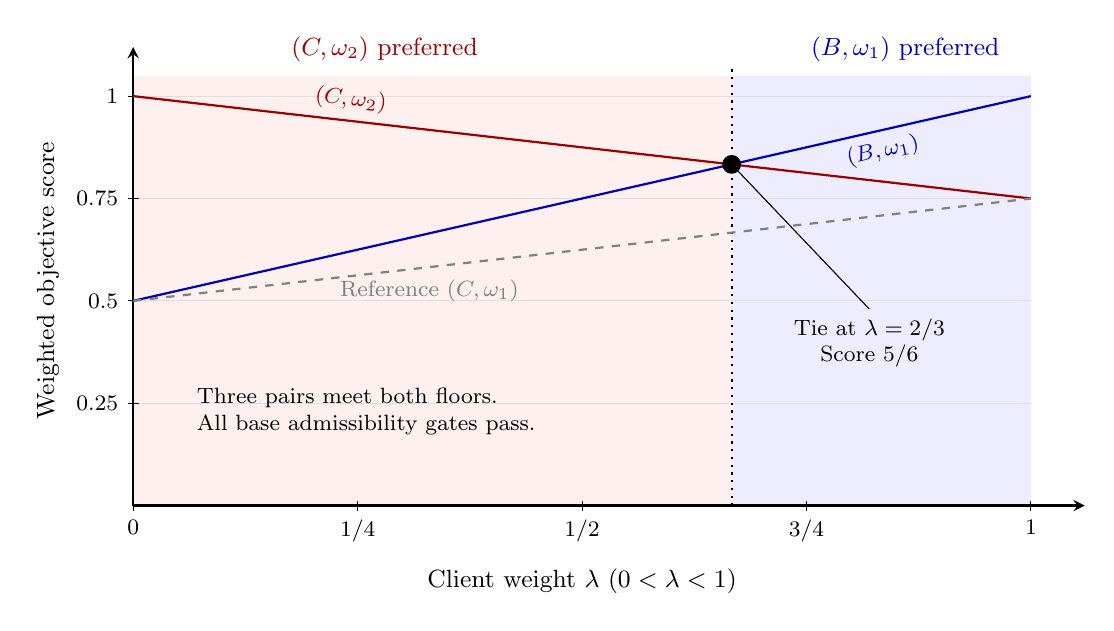
\begin{tikzpicture}[x=11.4cm,y=5.2cm,font=\small,>=stealth]
  \fill[red!6] (0,0) rectangle ({2/3},1.05);
  \fill[blue!7] ({2/3},0) rectangle (1,1.05);
  \foreach \v in {0.25,0.5,0.75,1} {
    \draw[gray!25] (0,\v) -- (1,\v);
    \draw (0.006,\v) -- (-0.006,\v) node[left,font=\footnotesize] {\v};
  }
  \draw[->,thick] (0,0) -- (1.06,0);
  \draw[->,thick] (0,0) -- (0,1.12);
  \foreach \v/\lab in {0/0,0.25/{1/4},0.5/{1/2},0.75/{3/4},1/1} {
    \draw (\v,0.012) -- (\v,-0.012) node[below,font=\footnotesize] {$\lab$};
  }
  \node[rotate=90] at (-0.095,0.55) {Weighted objective score};
  \node[below] at (0.5,-0.13) {Client weight $\lambda$ $(0<\lambda<1)$};
  \draw[dotted,thick] ({2/3},0) -- ({2/3},1.07);
  \draw[thick,red!60!black] (0,\JManagerCtwo) -- (1,\JClientCtwo);
  \draw[thick,blue!70!black] (0,\JManagerBone) -- (1,\JClientBone);
  \draw[thick,dashed,gray] (0,\JManagerCone) -- (1,\JClientCone);
  \node[above,text=red!60!black] at (0.28,1.06) {$(C,\omega_2)$ preferred};
  \node[above,text=blue!70!black] at (0.86,1.06) {$(B,\omega_1)$ preferred};
  \node[circle,fill=black,inner sep=2.4pt] at ({2/3},{5/6}) {};
  \draw[thin] ({2/3},{5/6}) -- (0.82,0.48);
  \node[anchor=north,align=center,font=\footnotesize] at (0.82,0.48)
    {Tie at $\lambda=2/3$\\Score $5/6$};
  \node[above,rotate=-6,text=red!60!black,font=\footnotesize] at (0.24,0.94) {$(C,\omega_2)$};
  \node[below,rotate=13,text=blue!70!black,font=\footnotesize] at (0.83,0.915) {$(B,\omega_1)$};
  \node[below,text=gray,font=\footnotesize] at (0.33,0.575) {Reference $(C,\omega_1)$};
  \node[anchor=north west,align=left,font=\footnotesize,text width=4.5cm] at (0.06,0.31)
    {Three pairs meet both floors.\\All base admissibility gates pass.};
\end{tikzpicture}
